\section[Cohomology of unitarizable modules for Cn, 1 < n < 4]{Cohomology for $C_n$, $2 \leq n \leq 3$}

\subsection[sp(2): 1, 1, 1]{$\boldsymbol{\mathfrak{sp}(2)\!:\; r = 1,\, q = 1,\, l = 1}$}

Cone of unitarizable weights: $\left(a_{1} + 2\right)\omega_{1} - \left(a_{1} + 3\right)\omega_{2}$ \\


\begin{figure}[H]
  \centering
      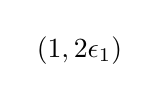
\begin{tikzpicture}[>=latex,line join=bevel,]
%%
\node (node_0) at (19.0bp,8.5bp) [draw,draw=none] {$(1, 2\epsilon_{1})$};
%
\end{tikzpicture}
  \caption{Nonnegative scalar products with noncompact roots}
\end{figure}
    

%\noindent $\lambda = $ $\left(a_{1} + 2\right)\omega_{1} - \left(a_{1} + 3\right)\omega_{2}$ \\
\noindent Set of singular roots: $\emptyset$ \\

\begin{figure}[H]
  \centering
  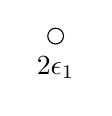
\begin{tikzpicture}
\draw[fill=white] (0 cm, 0 cm) circle (.1cm) node[below=4pt]{$2\epsilon_{1}$};
\end{tikzpicture}
  \caption{The reduced hermitian symmetric pair $(\mathfrak{g}_\lambda, \mathfrak{k}_\lambda)$}
\end{figure}

\begin{figure}[H]
  \centering
      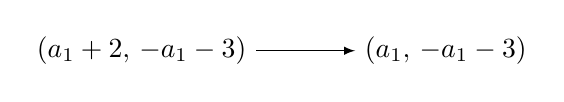
\begin{tikzpicture}[>=latex,line join=bevel,]
%%
\node (node_1) at (41.0bp,8.5bp) [draw,draw=none] {$\left(a_{1} + 2,\,-a_{1} - 3\right)$};
  \node (node_0) at (150.5bp,8.5bp) [draw,draw=none] {$\left(a_{1},\,-a_{1} - 3\right)$};
  \draw [black,->] (node_1) ..controls (90.432bp,8.5bp) and (99.314bp,8.5bp)  .. (node_0);
%
\end{tikzpicture}
  \caption{Nilpotent cohomology / BGG resolution}
\end{figure}

        


\subsection[sp(2): 2, 1, 1]{$\boldsymbol{\mathfrak{sp}(2)\!:\; r = 2,\, q = 1,\, l = 1}$}

Cone of unitarizable weights: $\omega_{1} - \frac{3}{2}\omega_{2}$ \\


\begin{figure}[H]
  \centering
      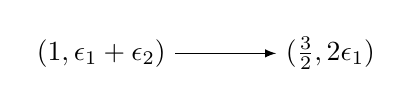
\begin{tikzpicture}[>=latex,line join=bevel,]
%%
\node (node_1) at (27.0bp,9.0bp) [draw,draw=none] {$(1, \epsilon_{1} + \epsilon_{2})$};
  \node (node_0) at (109.5bp,9.0bp) [draw,draw=none] {$(\frac{3}{2}, 2\epsilon_{1})$};
  \draw [black,->] (node_1) ..controls (62.548bp,9.0bp) and (71.612bp,9.0bp)  .. (node_0);
%
\end{tikzpicture}
  \caption{Nonnegative scalar products with noncompact roots}
\end{figure}
    

%\noindent $\lambda = $ $\omega_{1} - \frac{3}{2}\omega_{2}$ \\
\noindent Set of singular roots: $\emptyset$ \\

\begin{figure}[H]
  \centering
  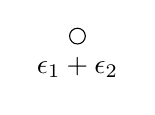
\begin{tikzpicture}
\draw[fill=white] (0 cm, 0 cm) circle (.1cm) node[below=4pt]{$\epsilon_{1} + \epsilon_{2}$};
\end{tikzpicture}
  \caption{The reduced hermitian symmetric pair $(\mathfrak{g}_\lambda, \mathfrak{k}_\lambda)$}
\end{figure}

\begin{figure}[H]
  \centering
      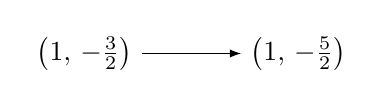
\begin{tikzpicture}[>=latex,line join=bevel,]
%%
\node (node_1) at (97.5bp,9.5bp) [draw,draw=none] {$\left(1,\,-\frac{5}{2}\right)$};
  \node (node_0) at (20.5bp,9.5bp) [draw,draw=none] {$\left(1,\,-\frac{3}{2}\right)$};
  \draw [black,->] (node_0) ..controls (49.043bp,9.5bp) and (58.23bp,9.5bp)  .. (node_1);
%
\end{tikzpicture}
  \caption{Nilpotent cohomology / BGG resolution}
\end{figure}

        


\subsection[sp(2): 2, 2, 1]{$\boldsymbol{\mathfrak{sp}(2)\!:\; r = 2,\, q = 2,\, l = 1}$}

Cone of unitarizable weights: $0$ \\


\begin{figure}[H]
  \centering
      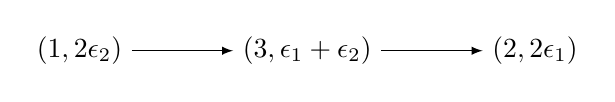
\begin{tikzpicture}[>=latex,line join=bevel,]
%%
\node (node_2) at (183.0bp,8.5bp) [draw,draw=none] {$(2, 2\epsilon_{1})$};
  \node (node_1) at (19.0bp,8.5bp) [draw,draw=none] {$(1, 2\epsilon_{2})$};
  \node (node_0) at (101.0bp,8.5bp) [draw,draw=none] {$(3, \epsilon_{1} + \epsilon_{2})$};
  \draw [black,->] (node_0) ..controls (136.4bp,8.5bp) and (145.48bp,8.5bp)  .. (node_2);
  \draw [black,->] (node_1) ..controls (45.708bp,8.5bp) and (54.762bp,8.5bp)  .. (node_0);
%
\end{tikzpicture}
  \caption{Nonnegative scalar products with noncompact roots}
\end{figure}
    

%\noindent $\lambda = $ $0$ \\
\noindent Set of singular roots: $\emptyset$ \\

\begin{figure}[H]
  \centering
  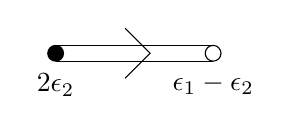
\begin{tikzpicture}
\draw (0 cm,0) -- (0 cm,0);
\draw (0 cm, 0.1 cm) -- +(2 cm,0);
\draw (0 cm, -0.1 cm) -- +(2 cm,0);
\draw[shift={(1.2, 0)}, rotate=0] (135 : 0.45cm) -- (0,0) -- (-135 : 0.45cm);
\draw[fill=black] (0 cm, 0 cm) circle (.1cm) node[below=4pt]{$2\epsilon_{2}$};
\draw[fill=white] (2 cm, 0 cm) circle (.1cm) node[below=4pt]{$\epsilon_{1} - \epsilon_{2}$};
\end{tikzpicture}
  \caption{The reduced hermitian symmetric pair $(\mathfrak{g}_\lambda, \mathfrak{k}_\lambda)$}
\end{figure}

\begin{figure}[H]
  \centering
      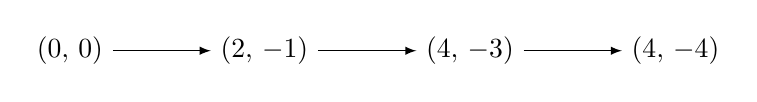
\begin{tikzpicture}[>=latex,line join=bevel,]
%%
\node (node_3) at (85.0bp,8.5bp) [draw,draw=none] {$\left(2,\,-1\right)$};
  \node (node_2) at (233.0bp,8.5bp) [draw,draw=none] {$\left(4,\,-4\right)$};
  \node (node_1) at (15.0bp,8.5bp) [draw,draw=none] {$\left(0,\,0\right)$};
  \node (node_0) at (159.0bp,8.5bp) [draw,draw=none] {$\left(4,\,-3\right)$};
  \draw [black,->] (node_1) ..controls (37.527bp,8.5bp) and (46.927bp,8.5bp)  .. (node_3);
  \draw [black,->] (node_3) ..controls (111.87bp,8.5bp) and (121.03bp,8.5bp)  .. (node_0);
  \draw [black,->] (node_0) ..controls (185.87bp,8.5bp) and (195.03bp,8.5bp)  .. (node_2);
%
\end{tikzpicture}
  \caption{Nilpotent cohomology / BGG resolution}
\end{figure}

        


\subsection[sp(2): 2, 2, 2]{$\boldsymbol{\mathfrak{sp}(2)\!:\; r = 2,\, q = 2,\, l = 2}$}

Cone of unitarizable weights: $-\frac{1}{2}\omega_{2}$ \\


\begin{figure}[H]
  \centering
      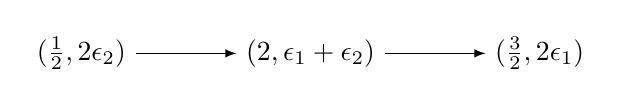
\begin{tikzpicture}[>=latex,line join=bevel,]
%%
\node (node_2) at (19.5bp,9.0bp) [draw,draw=none] {$(\frac{1}{2}, 2\epsilon_{2})$};
  \node (node_1) at (102.0bp,9.0bp) [draw,draw=none] {$(2, \epsilon_{1} + \epsilon_{2})$};
  \node (node_0) at (184.5bp,9.0bp) [draw,draw=none] {$(\frac{3}{2}, 2\epsilon_{1})$};
  \draw [black,->] (node_2) ..controls (46.782bp,9.0bp) and (55.855bp,9.0bp)  .. (node_1);
  \draw [black,->] (node_1) ..controls (137.55bp,9.0bp) and (146.61bp,9.0bp)  .. (node_0);
%
\end{tikzpicture}
  \caption{Nonnegative scalar products with noncompact roots}
\end{figure}
    

%\noindent $\lambda = $ $-\frac{1}{2}\omega_{2}$ \\
\noindent Set of singular roots: $\emptyset$ \\

\begin{figure}[H]
  \centering
  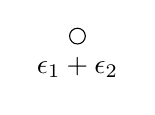
\begin{tikzpicture}
\draw[fill=white] (0 cm, 0 cm) circle (.1cm) node[below=4pt]{$\epsilon_{1} + \epsilon_{2}$};
\end{tikzpicture}
  \caption{The reduced hermitian symmetric pair $(\mathfrak{g}_\lambda, \mathfrak{k}_\lambda)$}
\end{figure}

\begin{figure}[H]
  \centering
      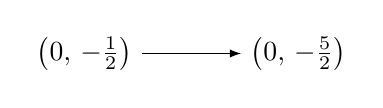
\begin{tikzpicture}[>=latex,line join=bevel,]
%%
\node (node_1) at (97.5bp,9.5bp) [draw,draw=none] {$\left(0,\,-\frac{5}{2}\right)$};
  \node (node_0) at (20.5bp,9.5bp) [draw,draw=none] {$\left(0,\,-\frac{1}{2}\right)$};
  \draw [black,->] (node_0) ..controls (49.043bp,9.5bp) and (58.23bp,9.5bp)  .. (node_1);
%
\end{tikzpicture}
  \caption{Nilpotent cohomology / BGG resolution}
\end{figure}

        


\subsection[sp(3): 1, 1, 1]{$\boldsymbol{\mathfrak{sp}(3)\!:\; r = 1,\, q = 1,\, l = 1}$}

Cone of unitarizable weights: $\left(a_{1} + 2\right)\omega_{1} + a_2\omega_2 - \left(a_{1} + a_{2} + 4\right)\omega_{3}$ \\


\begin{figure}[H]
  \centering
      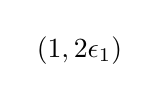
\begin{tikzpicture}[>=latex,line join=bevel,]
%%
\node (node_0) at (19.0bp,8.5bp) [draw,draw=none] {$(1, 2\epsilon_{1})$};
%
\end{tikzpicture}
  \caption{Nonnegative scalar products with noncompact roots}
\end{figure}
    

%\noindent $\lambda = $ $\left(a_{1} + 2\right)\omega_{1} - \left(a_{1} + a_{2} + 4\right)\omega_{3}$ \\
\noindent Set of singular roots: $\emptyset$ \\

\begin{figure}[H]
  \centering
  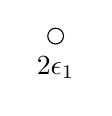
\begin{tikzpicture}
\draw[fill=white] (0 cm, 0 cm) circle (.1cm) node[below=4pt]{$2\epsilon_{1}$};
\end{tikzpicture}
  \caption{The reduced Hermitian symmetric pair $(\mathfrak{g}_\lambda, \mathfrak{k}_\lambda)$}
\end{figure}

\begin{figure}[H]
  \centering
      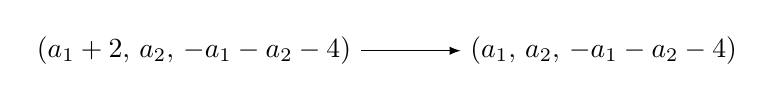
\begin{tikzpicture}[>=latex,line join=bevel,]
%%
\node (node_1) at (60.0bp,8.5bp) [draw,draw=none] {$\left(a_{1} + 2,\,a_{2},\,-a_{1} - a_{2} - 4\right)$};
  \node (node_0) at (207.5bp,8.5bp) [draw,draw=none] {$\left(a_{1},\,a_{2},\,-a_{1} - a_{2} - 4\right)$};
  \draw [black,->] (node_1) ..controls (128.57bp,8.5bp) and (137.21bp,8.5bp)  .. (node_0);
%
\end{tikzpicture}
  \caption{Nilpotent cohomology / BGG resolution}
\end{figure}

        


\subsection[sp(3): 2, 1, 1]{$\boldsymbol{\mathfrak{sp}(3)\!:\; r = 2,\, q = 1,\, l = 1}$}

Cone of unitarizable weights: $\omega_{1} + \left(a_{2} + 1\right)\omega_{2} - \left(a_{2} + \frac{7}{2}\right)\omega_{3}$ \\


\begin{figure}[H]
  \centering
      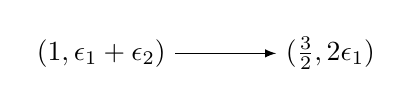
\begin{tikzpicture}[>=latex,line join=bevel,]
%%
\node (node_1) at (27.0bp,9.0bp) [draw,draw=none] {$(1, \epsilon_{1} + \epsilon_{2})$};
  \node (node_0) at (109.5bp,9.0bp) [draw,draw=none] {$(\frac{3}{2}, 2\epsilon_{1})$};
  \draw [black,->] (node_1) ..controls (62.548bp,9.0bp) and (71.612bp,9.0bp)  .. (node_0);
%
\end{tikzpicture}
  \caption{Nonnegative scalar products with noncompact roots}
\end{figure}
    

%\noindent $\lambda = $ $\omega_{1} + \left(a_{2} + 1\right)\omega_{2} - \left(a_{2} + \frac{7}{2}\right)\omega_{3}$ \\
\noindent Set of singular roots: $\emptyset$ \\

\begin{figure}[H]
  \centering
  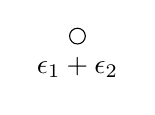
\begin{tikzpicture}
\draw[fill=white] (0 cm, 0 cm) circle (.1cm) node[below=4pt]{$\epsilon_{1} + \epsilon_{2}$};
\end{tikzpicture}
  \caption{The reduced Hermitian symmetric pair $(\mathfrak{g}_\lambda, \mathfrak{k}_\lambda)$}
\end{figure}

\begin{figure}[H]
  \centering
      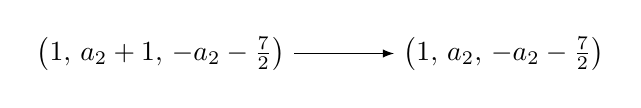
\begin{tikzpicture}[>=latex,line join=bevel,]
%%
\node (node_1) at (48.0bp,9.5bp) [draw,draw=none] {$\left(1,\,a_{2} + 1,\,-a_{2} - \frac{7}{2}\right)$};
  \node (node_0) at (171.5bp,9.5bp) [draw,draw=none] {$\left(1,\,a_{2},\,-a_{2} - \frac{7}{2}\right)$};
  \draw [black,->] (node_1) ..controls (104.66bp,9.5bp) and (113.35bp,9.5bp)  .. (node_0);
%
\end{tikzpicture}
  \caption{Nilpotent cohomology / BGG resolution}
\end{figure}

        


\subsection[sp(3): 2, 2, 1]{$\boldsymbol{\mathfrak{sp}(3)\!:\; r = 2,\, q = 2,\, l = 1}$}

Cone of unitarizable weights: $\left(a_{2} + 2\right)\omega_{2} - \left(a_{2} + 3\right)\omega_{3}$ \\


\begin{figure}[H]
  \centering
      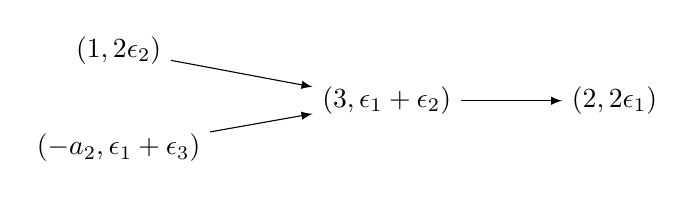
\begin{tikzpicture}[>=latex,line join=bevel,]
%%
\node (node_3) at (33.5bp,8.5bp) [draw,draw=none] {$(-a_{2}, \epsilon_{1} + \epsilon_{3})$};
  \node (node_2) at (212.0bp,25.5bp) [draw,draw=none] {$(2, 2\epsilon_{1})$};
  \node (node_1) at (33.5bp,43.5bp) [draw,draw=none] {$(1, 2\epsilon_{2})$};
  \node (node_0) at (130.0bp,25.5bp) [draw,draw=none] {$(3, \epsilon_{1} + \epsilon_{2})$};
  \draw [black,->] (node_3) ..controls (75.372bp,15.853bp) and (84.404bp,17.478bp)  .. (node_0);
  \draw [black,->] (node_0) ..controls (165.4bp,25.5bp) and (174.48bp,25.5bp)  .. (node_2);
  \draw [black,->] (node_1) ..controls (64.089bp,37.864bp) and (79.119bp,35.001bp)  .. (node_0);
%
\end{tikzpicture}
  \caption{Nonnegative scalar products with noncompact roots}
\end{figure}
    

\noindent $\lambda = 2\omega_{2} - 3\omega_{3}$ \\
\noindent Set of singular roots: $\{\epsilon_{1} + \epsilon_{3}$\} \\

\begin{figure}[H]
  \centering
  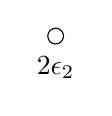
\begin{tikzpicture}
\draw[fill=white] (0 cm, 0 cm) circle (.1cm) node[below=4pt]{$2\epsilon_{2}$};
\end{tikzpicture}
  \caption{The reduced Hermitian symmetric pair $(\mathfrak{g}_\lambda, \mathfrak{k}_\lambda)$}
\end{figure}

\begin{figure}[H]
  \centering
      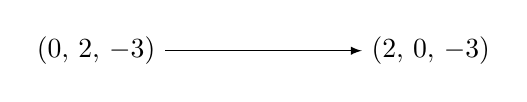
\begin{tikzpicture}[>=latex,line join=bevel,]
%%
\node (node_1) at (46.5bp,8.5bp) [draw,draw=none] {$\left(0,\,  2,\,- 3\right)$};
  \node (node_0) at (167.0bp,8.5bp) [draw,draw=none] {$\left(2,\,0,\, - 3\right)$};
  \draw [black,->] (node_1) ..controls (101.65bp,8.5bp) and (110.36bp,8.5bp)  .. (node_0);
%
\end{tikzpicture}
  \caption{Nilpotent cohomology / BGG resolution}
\end{figure}

\noindent $\lambda = \left(a_{2} + 2\right)\omega_{2} - \left(a_{2} + 3\right)\omega_{3}$, $a_2\geq 1$ \\
\noindent Set of singular roots: $\emptyset$ \\

\begin{figure}[H]
  \centering
  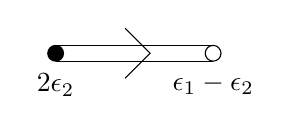
\begin{tikzpicture}
\draw (0 cm,0) -- (0 cm,0);
\draw (0 cm, 0.1 cm) -- +(2 cm,0);
\draw (0 cm, -0.1 cm) -- +(2 cm,0);
\draw[shift={(1.2, 0)}, rotate=0] (135 : 0.45cm) -- (0,0) -- (-135 : 0.45cm);
\draw[fill=black] (0 cm, 0 cm) circle (.1cm) node[below=4pt]{$2\epsilon_{2}$};
\draw[fill=white] (2 cm, 0 cm) circle (.1cm) node[below=4pt]{$\epsilon_{1} - \epsilon_{2}$};
\end{tikzpicture}
  \caption{The reduced Hermitian symmetric pair $(\mathfrak{g}_\lambda, \mathfrak{k}_\lambda)$}
\end{figure}

\begin{figure}[H]
  \centering
      \begin{tikzpicture}[>=latex,line join=bevel,]
%%
 \node (node_0) at (0,3) [draw,draw=none] {$\left(0,\,a_{2} + 2,\,-a_{2} - 3\right)$};
 \node (node_1) at (3,2) [draw,draw=none] {$\left(2,\,a_{2} + 1,\,-a_{2} - 3\right)$};
 \node (node_2) at (6,1) [draw,draw=none] {$\left(4,\,a_{2} - 1,\,-a_{2} - 3\right)$};
 \node (node_3) at (9,0) [draw,draw=none] {$\left(4,\,a_{2} - 2,\,-a_{2} - 3\right)$};
 
  \draw [black,->] (node_0) edge (node_1);
  \draw [black,->] (node_1) edge (node_2);
  \draw [black,->] (node_2) edge (node_3);
%
\end{tikzpicture}
  \caption{Nilpotent cohomology / BGG resolution}
\end{figure}        


\subsection[sp(3): 2, 2, 2]{$\boldsymbol{\mathfrak{sp}(3)\!:\; r = 2,\, q = 2,\, l = 2}$}

Cone of unitarizable weights: $\left(a_{2} + 2\right)\omega_{2} - \left(a_{2} + \frac{7}{2}\right)\omega_{3}$ \\


\begin{figure}[H]
  \centering
      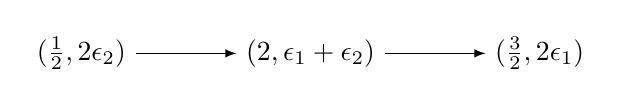
\begin{tikzpicture}[>=latex,line join=bevel,]
%%
\node (node_2) at (184.5bp,9.0bp) [draw,draw=none] {$(\frac{3}{2}, 2\epsilon_{1})$};
  \node (node_1) at (19.5bp,9.0bp) [draw,draw=none] {$(\frac{1}{2}, 2\epsilon_{2})$};
  \node (node_0) at (102.0bp,9.0bp) [draw,draw=none] {$(2, \epsilon_{1} + \epsilon_{2})$};
  \draw [black,->] (node_0) ..controls (137.55bp,9.0bp) and (146.61bp,9.0bp)  .. (node_2);
  \draw [black,->] (node_1) ..controls (46.782bp,9.0bp) and (55.855bp,9.0bp)  .. (node_0);
%
\end{tikzpicture}
  \caption{Nonnegative scalar products with noncompact roots}
\end{figure}
    

%\noindent $\lambda = $ $\left(a_{2} + 2\right)\omega_{2} - \left(a_{2} + \frac{7}{2}\right)\omega_{3}$ \\
\noindent Set of singular roots: $\emptyset$ \\

\begin{figure}[H]
  \centering
  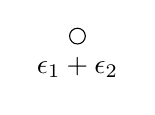
\begin{tikzpicture}
\draw[fill=white] (0 cm, 0 cm) circle (.1cm) node[below=4pt]{$\epsilon_{1} + \epsilon_{2}$};
\end{tikzpicture}
  \caption{The reduced Hermitian symmetric pair $(\mathfrak{g}_\lambda, \mathfrak{k}_\lambda)$}
\end{figure}

\begin{figure}[H]
  \centering
      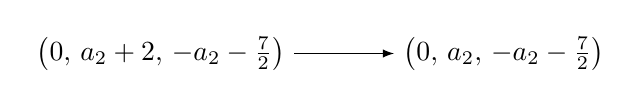
\begin{tikzpicture}[>=latex,line join=bevel,]
%%
\node (node_1) at (171.5bp,9.5bp) [draw,draw=none] {$\left(0,\,a_{2},\,-a_{2} - \frac{7}{2}\right)$};
  \node (node_0) at (48.0bp,9.5bp) [draw,draw=none] {$\left(0,\,a_{2} + 2,\,-a_{2} - \frac{7}{2}\right)$};
  \draw [black,->] (node_0) ..controls (104.66bp,9.5bp) and (113.35bp,9.5bp)  .. (node_1);
%
\end{tikzpicture}
  \caption{Nilpotent cohomology / BGG resolution}
\end{figure}

        


\subsection[sp(3): 3, 1, 1]{$\boldsymbol{\mathfrak{sp}(3)\!:\; r = 3,\, q = 1,\, l = 1}$}

Cone of unitarizable weights: $\omega_{1} - 2\omega_{3}$ \\


\begin{figure}[H]
  \centering
      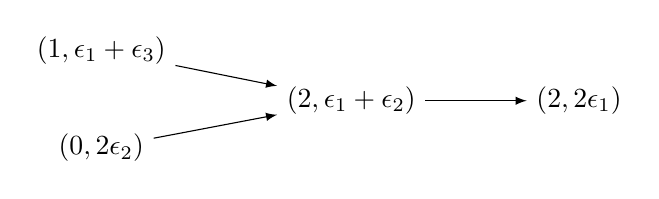
\begin{tikzpicture}[>=latex,line join=bevel,]
%%
\node (node_3) at (199.0bp,25.5bp) [draw,draw=none] {$(2, 2\epsilon_{1})$};
  \node (node_2) at (27.0bp,43.5bp) [draw,draw=none] {$(1, \epsilon_{1} + \epsilon_{3})$};
  \node (node_1) at (117.0bp,25.5bp) [draw,draw=none] {$(2, \epsilon_{1} + \epsilon_{2})$};
  \node (node_0) at (27.0bp,8.5bp) [draw,draw=none] {$(0, 2\epsilon_{2})$};
  \draw [black,->] (node_2) ..controls (62.481bp,36.447bp) and (71.507bp,34.601bp)  .. (node_1);
  \draw [black,->] (node_1) ..controls (152.4bp,25.5bp) and (161.48bp,25.5bp)  .. (node_3);
  \draw [black,->] (node_0) ..controls (55.968bp,13.903bp) and (68.3bp,16.285bp)  .. (node_1);
%
\end{tikzpicture}
  \caption{Nonnegative scalar products with noncompact roots}
\end{figure}
    

%\noindent $\lambda = $ $\omega_{1} - 2\omega_{3}$ \\
\noindent Set of singular roots: $\{2\epsilon_{2}$\} \\

\begin{figure}[H]
  \centering
  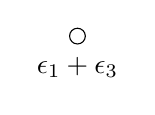
\begin{tikzpicture}
\draw[fill=white] (0 cm, 0 cm) circle (.1cm) node[below=4pt]{$\epsilon_{1} + \epsilon_{3}$};
\end{tikzpicture}
  \caption{The reduced Hermitian symmetric pair $(\mathfrak{g}_\lambda, \mathfrak{k}_\lambda)$}
\end{figure}

\begin{figure}[H]
  \centering
      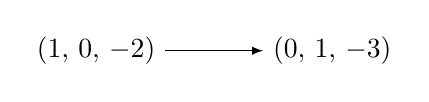
\begin{tikzpicture}[>=latex,line join=bevel,]
%%
\node (node_1) at (109.5bp,8.5bp) [draw,draw=none] {$\left(0,\,1,\,-3\right)$};
  \node (node_0) at (24.5bp,8.5bp) [draw,draw=none] {$\left(1,\,0,\,-2\right)$};
  \draw [black,->] (node_0) ..controls (57.035bp,8.5bp) and (66.102bp,8.5bp)  .. (node_1);
%
\end{tikzpicture}
  \caption{Nilpotent cohomology / BGG resolution}
\end{figure}

        


\subsection[sp(3): 3, 2, 1]{$\boldsymbol{\mathfrak{sp}(3)\!:\; r = 3,\, q = 2,\, l = 1}$}

Cone of unitarizable weights: $\omega_{2} - \frac{3}{2}\omega_{3}$ \\


\begin{figure}[H]
  \centering
      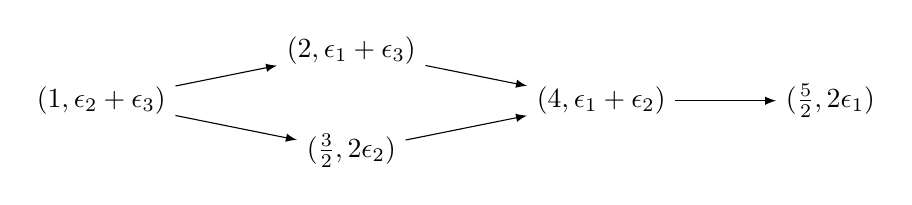
\begin{tikzpicture}[>=latex,line join=bevel,]
%%
\node (node_4) at (117.0bp,45.0bp) [draw,draw=none] {$(2, \epsilon_{1} + \epsilon_{3})$};
  \node (node_3) at (117.0bp,9.0bp) [draw,draw=none] {$(\frac{3}{2}, 2\epsilon_{2})$};
  \node (node_2) at (27.0bp,27.0bp) [draw,draw=none] {$(1, \epsilon_{2} + \epsilon_{3})$};
  \node (node_1) at (207.0bp,27.0bp) [draw,draw=none] {$(4, \epsilon_{1} + \epsilon_{2})$};
  \node (node_0) at (289.5bp,27.0bp) [draw,draw=none] {$(\frac{5}{2}, 2\epsilon_{1})$};
  \draw [black,->] (node_2) ..controls (64.807bp,19.471bp) and (76.782bp,17.022bp)  .. (node_3);
  \draw [black,->] (node_1) ..controls (242.55bp,27.0bp) and (251.61bp,27.0bp)  .. (node_0);
  \draw [black,->] (node_3) ..controls (146.24bp,14.777bp) and (158.25bp,17.233bp)  .. (node_1);
  \draw [black,->] (node_4) ..controls (152.48bp,37.947bp) and (161.51bp,36.101bp)  .. (node_1);
  \draw [black,->] (node_2) ..controls (62.481bp,34.053bp) and (71.507bp,35.899bp)  .. (node_4);
%
\end{tikzpicture}
  \caption{Nonnegative scalar products with noncompact roots}
\end{figure}
    

%\noindent $\lambda = $ $\omega_{2} - \frac{3}{2}\omega_{3}$ \\
\noindent Set of singular roots: $\emptyset$ \\

\begin{figure}[H]
  \centering
  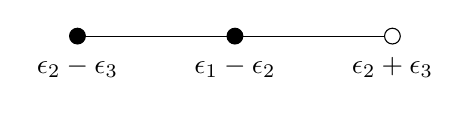
\begin{tikzpicture}
\draw (0 cm,0) -- (4 cm,0);
\draw[fill=black] (0 cm, 0 cm) circle (.1cm) node[below=4pt]{$\epsilon_{2} - \epsilon_{3}$};
\draw[fill=black] (2 cm, 0 cm) circle (.1cm) node[below=4pt]{$\epsilon_{1} - \epsilon_{2}$};
\draw[fill=white] (4 cm, 0 cm) circle (.1cm) node[below=4pt]{$\epsilon_{2} + \epsilon_{3}$};
\end{tikzpicture}
  \caption{The reduced Hermitian symmetric pair $(\mathfrak{g}_\lambda, \mathfrak{k}_\lambda)$}
\end{figure}

\begin{figure}[H]
  \centering
      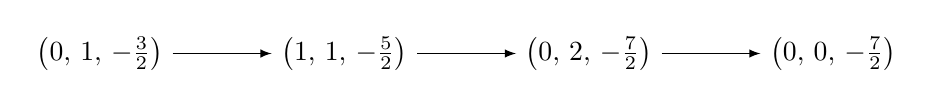
\begin{tikzpicture}[>=latex,line join=bevel,]
%%
\node (node_3) at (202.0bp,9.5bp) [draw,draw=none] {$\left(0,\,2,\,-\frac{7}{2}\right)$};
  \node (node_2) at (114.0bp,9.5bp) [draw,draw=none] {$\left(1,\,1,\,-\frac{5}{2}\right)$};
  \node (node_1) at (26.0bp,9.5bp) [draw,draw=none] {$\left(0,\,1,\,-\frac{3}{2}\right)$};
  \node (node_0) at (290.0bp,9.5bp) [draw,draw=none] {$\left(0,\,0,\,-\frac{7}{2}\right)$};
  \draw [black,->] (node_3) ..controls (236.3bp,9.5bp) and (245.24bp,9.5bp)  .. (node_0);
  \draw [black,->] (node_2) ..controls (148.3bp,9.5bp) and (157.24bp,9.5bp)  .. (node_3);
  \draw [black,->] (node_1) ..controls (60.298bp,9.5bp) and (69.237bp,9.5bp)  .. (node_2);
%
\end{tikzpicture}
  \caption{Nilpotent cohomology / BGG resolution}
\end{figure}

        


\subsection[sp(3): 3, 2, 2]{$\boldsymbol{\mathfrak{sp}(3)\!:\; r = 3,\, q = 2,\, l = 2}$}

Cone of unitarizable weights: $\omega_{2} - 2\omega_{3}$ \\


\begin{figure}[H]
  \centering
      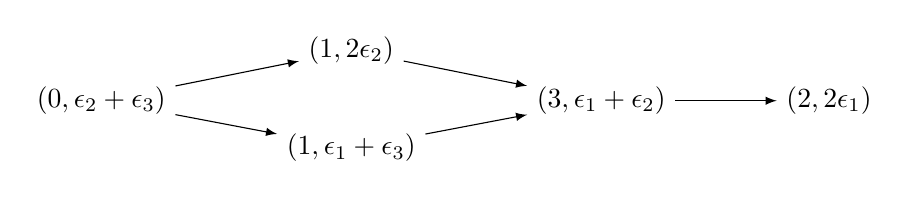
\begin{tikzpicture}[>=latex,line join=bevel,]
%%
\node (node_4) at (207.0bp,25.5bp) [draw,draw=none] {$(3, \epsilon_{1} + \epsilon_{2})$};
  \node (node_3) at (289.0bp,25.5bp) [draw,draw=none] {$(2, 2\epsilon_{1})$};
  \node (node_2) at (117.0bp,43.5bp) [draw,draw=none] {$(1, 2\epsilon_{2})$};
  \node (node_1) at (117.0bp,8.5bp) [draw,draw=none] {$(1, \epsilon_{1} + \epsilon_{3})$};
  \node (node_0) at (27.0bp,25.5bp) [draw,draw=none] {$(0, \epsilon_{2} + \epsilon_{3})$};
  \draw [black,->] (node_1) ..controls (152.39bp,15.144bp) and (161.31bp,16.867bp)  .. (node_4);
  \draw [black,->] (node_0) ..controls (62.393bp,18.856bp) and (71.311bp,17.133bp)  .. (node_1);
  \draw [black,->] (node_0) ..controls (64.959bp,33.06bp) and (77.132bp,35.55bp)  .. (node_2);
  \draw [black,->] (node_4) ..controls (242.4bp,25.5bp) and (251.48bp,25.5bp)  .. (node_3);
  \draw [black,->] (node_2) ..controls (145.97bp,37.779bp) and (158.3bp,35.257bp)  .. (node_4);
%
\end{tikzpicture}
  \caption{Nonnegative scalar products with noncompact roots}
\end{figure}
    

%\noindent $\lambda = $ $\omega_{2} - 2\omega_{3}$ \\
\noindent Set of singular roots: $\{\epsilon_{2} + \epsilon_{3}$\} \\

\begin{figure}[H]
  \centering
  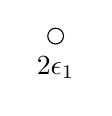
\begin{tikzpicture}
\draw[fill=white] (0 cm, 0 cm) circle (.1cm) node[below=4pt]{$2\epsilon_{1}$};
\end{tikzpicture}
  \caption{The reduced Hermitian symmetric pair $(\mathfrak{g}_\lambda, \mathfrak{k}_\lambda)$}
\end{figure}

\begin{figure}[H]
  \centering
      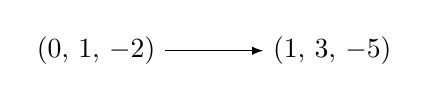
\begin{tikzpicture}[>=latex,line join=bevel,]
%%
\node (node_1) at (24.5bp,8.5bp) [draw,draw=none] {$\left(0,\,1,\,-2\right)$};
  \node (node_0) at (109.5bp,8.5bp) [draw,draw=none] {$\left(1,\,3,\,-5\right)$};
  \draw [black,->] (node_1) ..controls (57.035bp,8.5bp) and (66.102bp,8.5bp)  .. (node_0);
%
\end{tikzpicture}
  \caption{Nilpotent cohomology / BGG resolution}
\end{figure}

        


\subsection[sp(3): 3, 3, 1]{$\boldsymbol{\mathfrak{sp}(3)\!:\; r = 3,\, q = 3,\, l = 1}$}

Cone of unitarizable weights: $0$ \\


\begin{figure}[H]
  \centering
      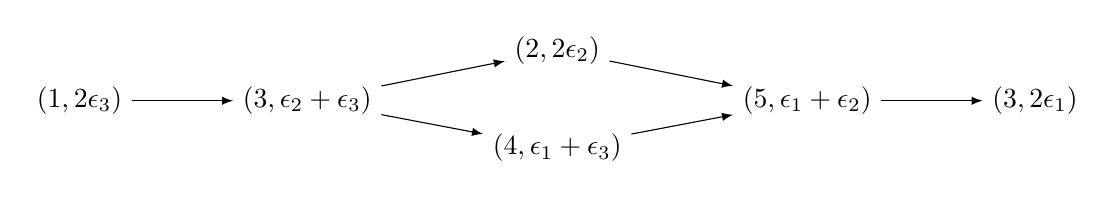
\begin{tikzpicture}[>=latex,line join=bevel,]
%%
\node (node_5) at (19.0bp,25.5bp) [draw,draw=none] {$(1, 2\epsilon_{3})$};
  \node (node_4) at (101.0bp,25.5bp) [draw,draw=none] {$(3, \epsilon_{2} + \epsilon_{3})$};
  \node (node_3) at (363.0bp,25.5bp) [draw,draw=none] {$(3, 2\epsilon_{1})$};
  \node (node_2) at (281.0bp,25.5bp) [draw,draw=none] {$(5, \epsilon_{1} + \epsilon_{2})$};
  \node (node_1) at (191.0bp,43.5bp) [draw,draw=none] {$(2, 2\epsilon_{2})$};
  \node (node_0) at (191.0bp,8.5bp) [draw,draw=none] {$(4, \epsilon_{1} + \epsilon_{3})$};
  \draw [black,->] (node_2) ..controls (316.4bp,25.5bp) and (325.48bp,25.5bp)  .. (node_3);
  \draw [black,->] (node_0) ..controls (226.39bp,15.144bp) and (235.31bp,16.867bp)  .. (node_2);
  \draw [black,->] (node_5) ..controls (45.708bp,25.5bp) and (54.762bp,25.5bp)  .. (node_4);
  \draw [black,->] (node_1) ..controls (219.97bp,37.779bp) and (232.3bp,35.257bp)  .. (node_2);
  \draw [black,->] (node_4) ..controls (138.96bp,33.06bp) and (151.13bp,35.55bp)  .. (node_1);
  \draw [black,->] (node_4) ..controls (136.39bp,18.856bp) and (145.31bp,17.133bp)  .. (node_0);
%
\end{tikzpicture}
  \caption{Nonnegative scalar products with noncompact roots}
\end{figure}
    

%\noindent $\lambda = $ $0$ \\
\noindent Set of singular roots: $\emptyset$ \\

\begin{figure}[H]
  \centering
  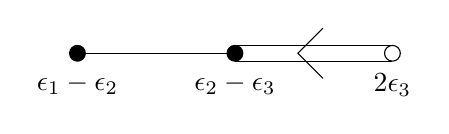
\begin{tikzpicture}
\draw (0 cm,0) -- (2 cm,0);
\draw (2 cm, 0.1 cm) -- +(2 cm,0);
\draw (2 cm, -0.1 cm) -- +(2 cm,0);
\draw[shift={(2.8, 0)}, rotate=180] (135 : 0.45cm) -- (0,0) -- (-135 : 0.45cm);
\draw[fill=black] (0 cm, 0 cm) circle (.1cm) node[below=4pt]{$\epsilon_{1} - \epsilon_{2}$};
\draw[fill=black] (2 cm, 0 cm) circle (.1cm) node[below=4pt]{$\epsilon_{2} - \epsilon_{3}$};
\draw[fill=white] (4 cm, 0 cm) circle (.1cm) node[below=4pt]{$2\epsilon_{3}$};
\end{tikzpicture}
  \caption{The reduced Hermitian symmetric pair $(\mathfrak{g}_\lambda, \mathfrak{k}_\lambda)$}
\end{figure}

\begin{figure}[H]
  \centering
      \begin{tikzpicture}[>=latex,line join=bevel,]
%%
\node (node_7) at (57.5bp,8.5bp) [draw,draw=none] {$\left(0,\,0,\,-4\right)$};
  \node (node_6) at (57.5bp,61.5bp) [draw,draw=none] {$\left(2,\,0,\,-4\right)$};
  \node (node_5) at (57.5bp,326.5bp) [draw,draw=none] {$\left(0,\,0,\,0\right)$};
  \node (node_4) at (57.5bp,273.5bp) [draw,draw=none] {$\left(0,\,2,\,-2\right)$};
  \node (node_3) at (91.5bp,167.5bp) [draw,draw=none] {$\left(3,\,0,\,-3\right)$};
  \node (node_2) at (57.5bp,220.5bp) [draw,draw=none] {$\left(1,\,2,\,-3\right)$};
  \node (node_1) at (57.5bp,114.5bp) [draw,draw=none] {$\left(2,\,1,\,-4\right)$};
  \node (node_0) at (24.5bp,167.5bp) [draw,draw=none] {$\left(0,\,3,\,-4\right)$};
  \draw [black,->] (node_2) ..controls (67.338bp,204.74bp) and (74.775bp,193.59bp)  .. (node_3);
  \draw [black,->] (node_5) ..controls (57.5bp,311.19bp) and (57.5bp,300.97bp)  .. (node_4);
  \draw [black,->] (node_3) ..controls (81.662bp,151.74bp) and (74.225bp,140.59bp)  .. (node_1);
  \draw [black,->] (node_6) ..controls (57.5bp,46.195bp) and (57.5bp,35.966bp)  .. (node_7);
  \draw [black,->] (node_2) ..controls (48.0bp,204.82bp) and (40.883bp,193.82bp)  .. (node_0);
  \draw [black,->] (node_0) ..controls (34.0bp,151.82bp) and (41.117bp,140.82bp)  .. (node_1);
  \draw [black,->] (node_1) ..controls (57.5bp,99.195bp) and (57.5bp,88.966bp)  .. (node_6);
  \draw [black,->] (node_4) ..controls (57.5bp,258.19bp) and (57.5bp,247.97bp)  .. (node_2);
%
\end{tikzpicture}
  \caption{Nilpotent cohomology / BGG resolution}
\end{figure}
        


\subsection[sp(3): 3, 3, 2]{$\boldsymbol{\mathfrak{sp}(3)\!:\; r = 3,\, q = 3,\, l = 2}$}

Cone of unitarizable weights: $-\frac{1}{2}\omega_{3}$ \\


\begin{figure}[H]
  \centering
      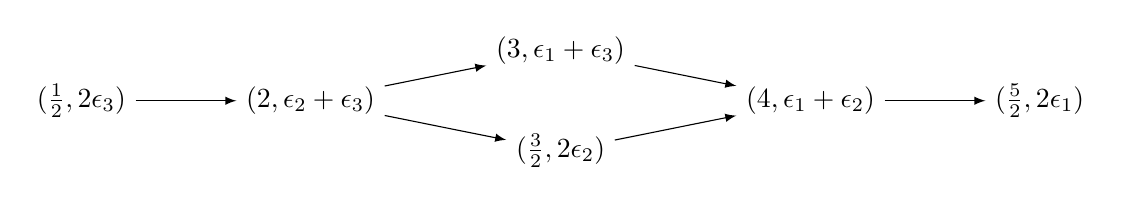
\begin{tikzpicture}[>=latex,line join=bevel,]
%%
\node (node_5) at (282.0bp,27.0bp) [draw,draw=none] {$(4, \epsilon_{1} + \epsilon_{2})$};
  \node (node_4) at (19.5bp,27.0bp) [draw,draw=none] {$(\frac{1}{2}, 2\epsilon_{3})$};
  \node (node_3) at (364.5bp,27.0bp) [draw,draw=none] {$(\frac{5}{2}, 2\epsilon_{1})$};
  \node (node_2) at (192.0bp,9.0bp) [draw,draw=none] {$(\frac{3}{2}, 2\epsilon_{2})$};
  \node (node_1) at (192.0bp,45.0bp) [draw,draw=none] {$(3, \epsilon_{1} + \epsilon_{3})$};
  \node (node_0) at (102.0bp,27.0bp) [draw,draw=none] {$(2, \epsilon_{2} + \epsilon_{3})$};
  \draw [black,->] (node_1) ..controls (227.48bp,37.947bp) and (236.51bp,36.101bp)  .. (node_5);
  \draw [black,->] (node_5) ..controls (317.55bp,27.0bp) and (326.61bp,27.0bp)  .. (node_3);
  \draw [black,->] (node_0) ..controls (139.81bp,19.471bp) and (151.78bp,17.022bp)  .. (node_2);
  \draw [black,->] (node_4) ..controls (46.782bp,27.0bp) and (55.855bp,27.0bp)  .. (node_0);
  \draw [black,->] (node_0) ..controls (137.48bp,34.053bp) and (146.51bp,35.899bp)  .. (node_1);
  \draw [black,->] (node_2) ..controls (221.24bp,14.777bp) and (233.25bp,17.233bp)  .. (node_5);
%
\end{tikzpicture}
  \caption{Nonnegative scalar products with noncompact roots}
\end{figure}
    

%\noindent $\lambda = $ $-\frac{1}{2}\omega_{3}$ \\
\noindent Set of singular roots: $\emptyset$ \\

\begin{figure}[H]
  \centering
  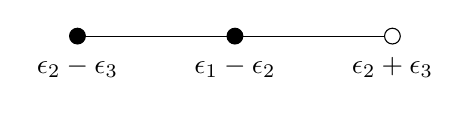
\begin{tikzpicture}
\draw (0 cm,0) -- (4 cm,0);
\draw[fill=black] (0 cm, 0 cm) circle (.1cm) node[below=4pt]{$\epsilon_{2} - \epsilon_{3}$};
\draw[fill=black] (2 cm, 0 cm) circle (.1cm) node[below=4pt]{$\epsilon_{1} - \epsilon_{2}$};
\draw[fill=white] (4 cm, 0 cm) circle (.1cm) node[below=4pt]{$\epsilon_{2} + \epsilon_{3}$};
\end{tikzpicture}
  \caption{The reduced Hermitian symmetric pair $(\mathfrak{g}_\lambda, \mathfrak{k}_\lambda)$}
\end{figure}

\begin{figure}[H]
  \centering
      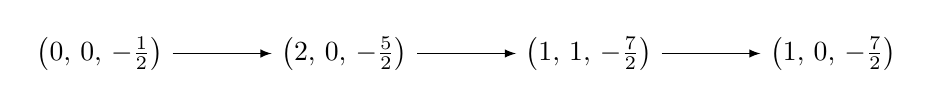
\begin{tikzpicture}[>=latex,line join=bevel,]
%%
\node (node_3) at (26.0bp,9.5bp) [draw,draw=none] {$\left(0,\,0,\,-\frac{1}{2}\right)$};
  \node (node_2) at (114.0bp,9.5bp) [draw,draw=none] {$\left(2,\,0,\,-\frac{5}{2}\right)$};
  \node (node_1) at (290.0bp,9.5bp) [draw,draw=none] {$\left(1,\,0,\,-\frac{7}{2}\right)$};
  \node (node_0) at (202.0bp,9.5bp) [draw,draw=none] {$\left(1,\,1,\,-\frac{7}{2}\right)$};
  \draw [black,->] (node_3) ..controls (60.298bp,9.5bp) and (69.237bp,9.5bp)  .. (node_2);
  \draw [black,->] (node_0) ..controls (236.3bp,9.5bp) and (245.24bp,9.5bp)  .. (node_1);
  \draw [black,->] (node_2) ..controls (148.3bp,9.5bp) and (157.24bp,9.5bp)  .. (node_0);
%
\end{tikzpicture}
  \caption{Nilpotent cohomology / BGG resolution}
\end{figure}

        


\subsection[sp(3): 3, 3, 3]{$\boldsymbol{\mathfrak{sp}(3)\!:\; r = 3,\, q = 3,\, l = 3}$}

Cone of unitarizable weights: $-\omega_{3}$ \\


\begin{figure}[H]
  \centering
      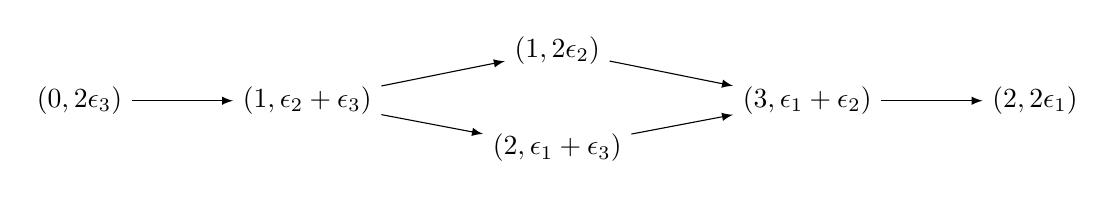
\begin{tikzpicture}[>=latex,line join=bevel,]
%%
\node (node_5) at (191.0bp,8.5bp) [draw,draw=none] {$(2, \epsilon_{1} + \epsilon_{3})$};
  \node (node_4) at (191.0bp,43.5bp) [draw,draw=none] {$(1, 2\epsilon_{2})$};
  \node (node_3) at (19.0bp,25.5bp) [draw,draw=none] {$(0, 2\epsilon_{3})$};
  \node (node_2) at (101.0bp,25.5bp) [draw,draw=none] {$(1, \epsilon_{2} + \epsilon_{3})$};
  \node (node_1) at (363.0bp,25.5bp) [draw,draw=none] {$(2, 2\epsilon_{1})$};
  \node (node_0) at (281.0bp,25.5bp) [draw,draw=none] {$(3, \epsilon_{1} + \epsilon_{2})$};
  \draw [black,->] (node_3) ..controls (45.708bp,25.5bp) and (54.762bp,25.5bp)  .. (node_2);
  \draw [black,->] (node_5) ..controls (226.39bp,15.144bp) and (235.31bp,16.867bp)  .. (node_0);
  \draw [black,->] (node_4) ..controls (219.97bp,37.779bp) and (232.3bp,35.257bp)  .. (node_0);
  \draw [black,->] (node_0) ..controls (316.4bp,25.5bp) and (325.48bp,25.5bp)  .. (node_1);
  \draw [black,->] (node_2) ..controls (136.39bp,18.856bp) and (145.31bp,17.133bp)  .. (node_5);
  \draw [black,->] (node_2) ..controls (138.96bp,33.06bp) and (151.13bp,35.55bp)  .. (node_4);
%
\end{tikzpicture}
  \caption{Nonnegative scalar products with noncompact roots}
\end{figure}
    

%\noindent $\lambda = $ $-\omega_{3}$ \\
\noindent Set of singular roots: $\{2\epsilon_{3}$\} \\

\begin{figure}[H]
  \centering
  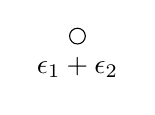
\begin{tikzpicture}
\draw[fill=white] (0 cm, 0 cm) circle (.1cm) node[below=4pt]{$\epsilon_{1} + \epsilon_{2}$};
\end{tikzpicture}
  \caption{The reduced Hermitian symmetric pair $(\mathfrak{g}_\lambda, \mathfrak{k}_\lambda)$}
\end{figure}

\begin{figure}[H]
  \centering
      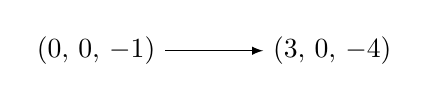
\begin{tikzpicture}[>=latex,line join=bevel,]
%%
\node (node_1) at (24.5bp,8.5bp) [draw,draw=none] {$\left(0,\,0,\,-1\right)$};
  \node (node_0) at (109.5bp,8.5bp) [draw,draw=none] {$\left(3,\,0,\,-4\right)$};
  \draw [black,->] (node_1) ..controls (57.035bp,8.5bp) and (66.102bp,8.5bp)  .. (node_0);
%
\end{tikzpicture}
  \caption{Nilpotent cohomology / BGG resolution}
\end{figure}
